\chapter{Spatially Random Maps}
\label{background}
As studying the effects of random spatial perturbations
on the dynamics of one-dimensional Maps may yield implications for
understanding the dynamics on higher dimensional maps, we present two
case studies:
\begin{enumerate}
\item the logistic map,
\item the circle map.
\end{enumerate}
The random spatial perturbations in both maps are intended to mimic
the noise used in hydraulic modeling for the porosity and hydraulic
conductivity, which is assumed to be log-normal with an
exponentially decaying spatial correlation. Observations
in subsurface hydrology suggest flow parameters are log-normal~\cite{gelhar}. The following sections
offer background information on the characteristics of both maps, with
and without random spatial perturbations. 
\section{Logistic Map}
\subsection{Deterministic case}
\hspace{5mm}The Logistic map is a quadratic recursive equation that maps the domain
$[0,1] \rightarrow [0,1]$. It is a commonly studied topic in nonlinear dynamics and has
applications in population modeling. Robert May popularized the
logistic map in 1976~\cite{may}. He demonstrated even simple nonlinear
maps could have complicated dynamics. There is one parameter in the
expression, $r$, which can take any value in the range [0,4] so that
[0,1] is an invariant set of the map. We define the map $f:[0,1]\to [0,1]$
\begin{equation}\label{logmap}
x_{n+1} = f(x_n) = rx_n(1-x_n).
\end{equation}
We require $[0,1]$ to be invariant in $f$ because of the stipulations
of the fixed point convergence theorem~\cite{atkinson}.
\begin{singlespace}
\begin{theorem}\label{thm:fp}
Let $D$ be a closed, bounded and convex set in the plane. Assume the
components of the iterative map $g(x)$ are continuously differentiable at all points of
$D$, and further assume: 
\begin{enumerate}
\item $g(D) \subset D$
\item $\lambda =\max_{x\in D}||G(x)||_\infty < 1$, where $G(x)$ is the Jacobian of
$g(x)$
\end{enumerate}
Then, 
\begin{itemize}
\item $x=g(x)$ has a unique solution $\alpha \in D$
\item For any initial point $x_0 \in D$, the iteration will converge
  in $D$, i.e. $\lim_{t \to \infty}x_t = \alpha$
\item $||\alpha - x_{n+1}||_\infty \leq
  (\lambda +\epsilon_n)||\alpha - x_n||_\infty$ with
  $\epsilon \to 0$ as $n\to \infty$
\end{itemize}
\end{theorem}
\end{singlespace}
 For a fixed initial condition $x_0$ and $r$, the long term behavior of
the map may be obtained by fixed point iteration, using~(\ref{logmap}). 
\begin{figure}[!h]
\caption[Deterministic logistic map, stable orbit]{Deterministic Logistic Map (blue) for $r=3.2$. There is a stable period
4 orbit. The period is calculated by counting the number
of crossings from the cobweb diagram (green) on the line $x_{n+1}=x_n$
(red). The transient iterations (the first 500) were removed to make
the long-term behavior of the orbit more obvious.}\label{fig:detlogstable}
    \begin{center}
	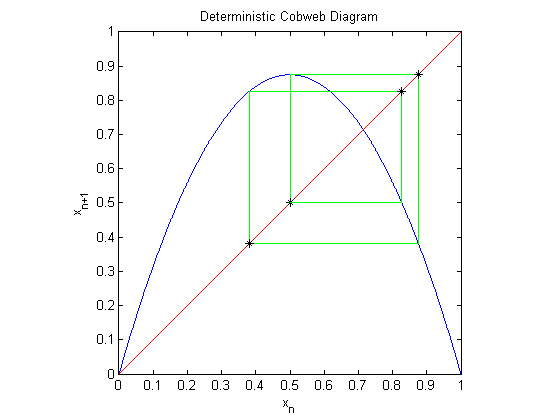
\includegraphics[scale=0.8]{figs/det_cobweb.png}
    \end{center}
\end{figure}
For example, Figure~\ref{fig:detlogstable}
demonstrates a stable period 4 orbit, whereas Figure~\ref{fig:detlogunstable}
demonstrates a possibly chaotic orbit. 
\begin{figure}[!h]
\caption[Deterministic logistic map, unstable orbit]{Deterministic
  Logistic Map (blue) for $r=3.8$. There appears to be no
  stable orbit. The cobweb diagram (green) behaves erratically, even
  after removing the transient behavior. For values of $r \in
  [3.5,4]$, the system is chaotic.}\label{fig:detlogunstable}
	\begin{center}
		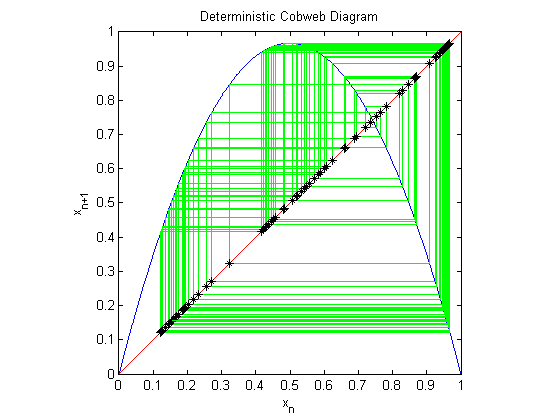
\includegraphics[scale=0.8]{figs/chaos.png}
	\end{center}
\end{figure} 
The effects of the parameter $r$ are
tabulated in Table~\ref{tbl:bif} and also graphically visualized in
Figure~\ref{fig:bif}. 
\begin {table}[!h]
\begin{center}
\caption[Behavior of the deterministic map as $r$ is varied]{As $r$ is
varied over [0,4], the logistic map undergoes notable changes in terms
of stability~\cite{may}.}\label{tbl:bif}
\begin{tabular}{ | p{4cm}| p{8cm}|}   \hline
$r \in [0,1]$ & convergence to the stable Period
1 orbit, $x=0$ \\ \hline
$r \in [1,2]$ & convergence to the stable Period 1
orbit, $x = \frac{r-1}{r}$\\ \hline
$r \in [2,3]$ & convergence to the stable Period 1
orbit, $x = \frac{r-1}{r}$, but at a slower rate\\ \hline
$r \in [3,3.44949]$ & emergence of stable Period 2 orbits\\ \hline
$r \in (3.44949, 3.54409)$ & emergence of stable Period 4 orbits\\ \hline
$r \in [3.54409,3.56995)$ & period doubling cascade\\ \hline
$ r \approx 3.56995 $ & onset of chaos\\\hline
$r \in (3.56995,4]$ & mostly chaotic behavior, but there are islands of
stability (eg. Period 3 orbits for $r \approx 3.82843$) \\\hline
\end{tabular}
\end{center}
\end {table}
Most notably, there is no chaos for values of $r
< 3.5$, and for $r > 3.5$, the system is mostly chaotic, although
there are islands of stability interspersed throughout the \textbf{bifurcation
diagram}. A bifurcation is a qualitative change in dynamics, such as
the creation or destruction of fixed points, or a change in their
stability~\cite{strogatz}. These changes are strongly dependent on the
parameters of the system. Therefore, a bifurcation diagram is a
visual demonstration of the change in dynamics of a system as its
parameters are varied. 
\begin{figure}[!h]
\caption[Bifurcation diagram for the deterministic logistic map]{The behavior in Table~\ref{tbl:bif} may be graphically represented
in a bifurcation diagram. The horizontal axis shows the value of $r$ as it ranges over
  $[0,4]$. The vertical axis plots the long term behavior of iterates
  in the deterministic logistic map. The left diagram ranges from $r\in
  [0,4]$, and the right diagram ranges from $r\in [2.5,4]$. Notice the
  islands of stability in the chaotic region of the map.}\label{fig:bif}
\centering
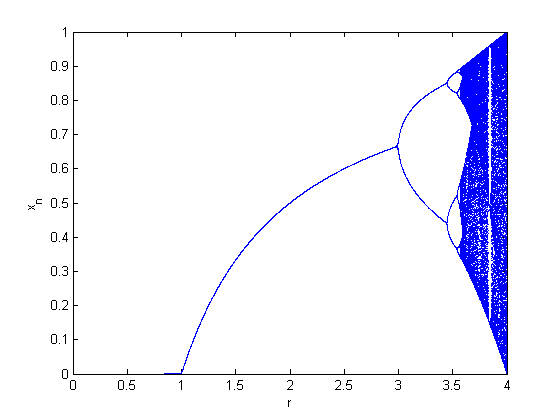
\includegraphics[width=.5\textwidth]{figs/det_bif_1.png}\hfill
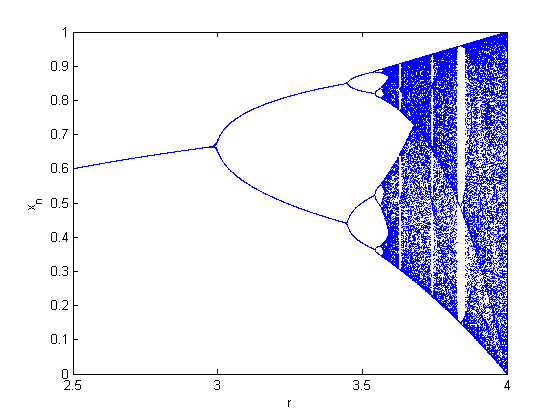
\includegraphics[width=.5\textwidth]{figs/det_bif_2.png}
\end{figure}
Bifurcation diagrams are constructed by
plotting the long term behavior of the map as a function of its
parameters. In the case of~(\ref{logmap}), we plot the
locations of the stable orbits as $r$ is varied over $[0,4]$.

\subsection{Random case}
The spatially random case has not been as well explored in the
literature as the temporally random case~\cite{athreya}. Athreya and
Dai explore the concept of a time-varying logistic map, where the
parameter $r_i$ is a function of each time step, as opposed to position
in space. At each time step, some $r_i \in \{r\}_0^\infty$ is applied
to the map, where the
sequence $\{r\}_0^\infty$ has independent and identically distributed
random variables in [0,4]. In contrast, the spatially random logistic
map replaces the parameter $r$ from~(\ref{logmap}) with a random
function of space, $R:[0,1]\to [0,4]$. As before, 
$f:[0,1]\to [0,1]$, where
\begin{equation}\label{randlogmap}
x_{n+1} = f(x_n) = R(x_n)x_n(1-x_n).
\end{equation}
Because the noise in hydraulic modeling is often assumed to be log-normal with an
exponentially decaying spatial correlation, we let
\begin{equation}\label{R}
\xi(x)=\ln(R(x)) 
\end{equation}
be a random variable~\cite{gelhar}. A normal distribution may be used
for subsurface storage properties\footnote{Some examples of subsurface
storage properties include porosity and moisture content.}, but in some cases, it is
inappropriate because it would imply negative values have nonzero
probability. Alternatively, a log-normal random variable~(\ref{R}) may
be used for physical parameters known to be nonnegative. Moreover, the log-normal distribution frequently appears when observing
nonnegative flow parameters underground, like hydraulic conductivity and
transmissivity~\cite{gelhar}. The mean $\mu$, variance $\sigma^2$, and
covariance (assuming homogeneity, so $C(x)$ is independent of $y$)
of~(\ref{R}) are defined as
\begin{align}
\begin{split}\label{cor}
\mu&=E[\xi(x)] = \ln(r)\\
\sigma^2&=E[(\xi(x) - \ln(r))^2]=E[\xi(x)^2]-(\ln(r))^2\\
C(x) &=E[(\xi(x+y) - E[\xi(x)])(\xi(y)-E[\xi(x)])] \\
&= E[(\xi(x+y) -\ln(r))(\xi(y)-\ln(r))]. 
\end{split}
\end{align}
The covariance function is usually a function of $x,y$, but if the
variability is independent of location in space, rather, dependent on the separation vector between the locations, we
call the covariance function
homogeneous~\cite{gelhar}. The noise in nonnegative flow parameters is
thought to rely on the distance between two points instead of their
precise locations, so $C(x)$ in (\ref{cor}) is
homogeneous. $C(x)$ is also called a correlation function, which
describes how variables at different positions in space are
related. It physically represents the degree of correlation between
two consecutive instances in the process. Correlations are strongest
when iterates are nearby, and they typically decay as the distance
between two iterates increases, although random processes could violate this assumption. 
Figure~\ref{fig:rlogstable} demonstrates one realization of the
spatially random logistic map.
\begin{figure}[!h]
\caption[Random logistic map, stable orbit]{One instance of a random
  logistic map (blue), which was iterated for 1000 steps. The map has converged to a stable period 4 orbit (green). Notice the
  ``wiggliness'' in the parabola shape. $r=3.5,L=0.05,N=200,\sigma=0.0061$}\label{fig:rlogstable}
	\begin{center}
		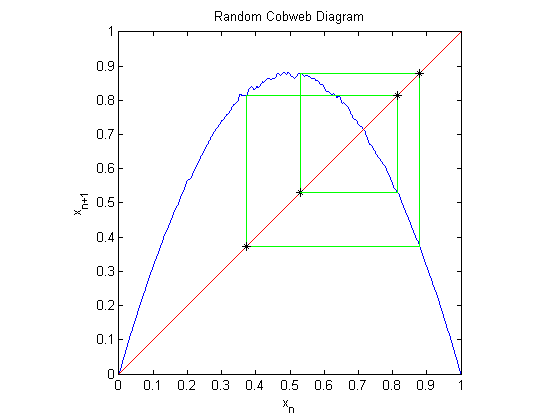
\includegraphics[scale=0.7]{figs/rand_cobweb.png}
	\end{center}
\end{figure}
We can construct such a
function $\xi(x)$ on $[0,1]$ that satisfies the above requirements with a Fourier
Series.
\begin{align}\label{fs1}
\begin{split}
\xi(x) &= \ln(r) + \sum_{n \in \mathbb{Z}}\hat{\xi_n}e^{2\pi inx}\\
\hat{\xi}_n &= a_n + ib_n = \hat{\xi}_{-n}^*
\end{split}
\end{align}
where the $*$ operator denotes the complex
conjugate. The requirement $\hat{\xi}_{-n}=\hat{\xi^*}_{n}$ ensures
$\xi(x) \in \mathbb{R}$. We can combine
the equations in~(\ref{fs1}) to arrive at the following form for
$\xi(x)$,
\begin{align}\label{fs2}
\xi(x) = \ln(r) + 2\sum^N_{n=1}a_n\cos(2\pi nx)-b_n\sin(2\pi nx),
\end{align}
where $N$ represents the number of Fourier modes in the sum, and is an
upper limit (necessary for numerical
simulations) that we impose on the summation.\footnote{In practice, $N
  \approx 10/L$, where $L$ represents the correlation length. $N$
  should be chosen to be large enough such that the Fourier amplitudes
may decay as more terms are included. This restriction will ensure the
fluctuations are log-normal.} (\ref{fs2}) assumes
$b_0=0$ to keep $\xi(x)$ in the real plane when $n=0$, and $a_0=0$
because we wish to maintain $E[\xi(x)]=\ln(r)$ when $n=0$ (the
spatially independent term $a_0$ will be absorbed into $\ln(r)$).
We can impose more restrictions of $|\hat{\xi}_n|$, the magnitude of
the Fourier modes. In particular,
we require the real and imaginary parts $(a_n,b_n)$ of $\hat{\xi}_n$
to be independent with mean $\hat{\mu}_n$ and variance $\hat{\sigma}^2_n$
\begin{align}
\begin{split}\label{Sn}
\hat{\mu}_n&=E[\hat{\xi}_n]=0\\
\hat{\sigma}_n^2&=E[\hat{\xi}_n^2]-(E[\hat{\xi}_n])^2=E[\hat{\xi}_n^2]\\
S(n)&=\hat{\sigma}_n^2,
\end{split}
\end{align}
where $S_n$ is the spectral density of the
log-fluctuations. (\ref{Sn}) represents the transformation of the
mean, variance, and covariance in~(\ref{cor}) to Fourier space. The
independent modes from the Fourier series have expectation
\begin{align*}
\begin{split}
E[\hat{\xi}_n\hat{\xi}_m]&=E[|\hat{\xi}_n||\hat{\xi}_n|\delta_{m+n}]\\
&=\delta_{m+n}E[|\hat{\xi}_n|^2]\\
&=\delta_{m+n}S(n).
\end{split}
\end{align*}
In other words, 
\begin{displaymath}
   E[\hat{\xi}_n\hat{\xi}_m] = \left\{
     \begin{array}{lr}
       \delta_{m+n}S(n) & : m = -n\\
       0 & : m \neq -n.\\
     \end{array}
   \right.
\end{displaymath} 
The spectral density $S(n)$ is defined as the Fourier transform of the
correlation function~(\ref{cor})~\cite{gelhar}
\begin{align*}
\begin{split}
\hat{C}(k) &= \int_{0}^{1}C(x)e^{-2\pi ikx}dx\\
&= \sum_{m,n} \int_{0}^{1} E[\hat{\xi}_n\hat{\xi}_m] e^{2\pi
  im(x+y)}e^{2\pi iny}e^{-2\pi ikx}dx\\
&=S(k).
\end{split}
\end{align*}
By nature of being defined as the Fourier transform of the covariance
function, the spectrum represents a distribution of variance over
frequency. In fact, for $x=0$, (\ref{cor}) reduces to the definition
of variance, so 
\begin{align*}
\begin{split}
C(x) &= \int_{-\infty}^{\infty}e^{ikx}S(k)\,dk\\
C(0) &= \sigma^2 = \int_{-\infty}^{\infty}S(k)\, dk.
\end{split}
\end{align*}
A simple spectrum that falls off quickly is
\begin{align}\label{spec}
S(n)=\alpha_n e^{-L|n|},
\end{align}
where $L \in [0,1]$ is the correlation length (and is fixed
for each simulation). Values of $L$ close to zero will result in a
small, negative exponent, which consequently increases the
spectrum. On the other hand, larger values of $L$ closer to one cause
the spectrum to decay faster. This choice of $S(n)$ corresponds to a correlation function
\begin{align}
\begin{split}
C(x) &= \sum_{n\in \mathbb{Z}}S(n)e^{2\pi inx}=\sum_{n\in \mathbb{Z}}\alpha \frac{1}{e^{L|n|}}e^{2\pi inx}\\
&= \alpha + \sum_{n=1}^{\infty}\alpha e^{2\pi
  inx-L|n|}+\sum_{n=-1}^{-\infty}\alpha e^{-2\pi inx-L|n|}\\
&= \alpha+\alpha \sum_{n=1}^{\infty}(e^{2\pi ix-L})^n+\alpha \sum_{m=1}^{\infty}(e^{-2\pi ix-L})^m\\
&=\alpha + \alpha \frac{e^{2\pi ix-L}}{1-e^{2\pi ix-L}} +\alpha
\frac{e^{-2\pi ix-L}}{1-e^{-2\pi ix-L}}\\
&=\alpha \left(1+ \frac{-2e^{-2L}+2\cos(2\pi x)e^{-L}}{e^{-2L}-2\cos(2\pi x)e^{-L}+1} \right).\\
\end{split}
\end{align}
Finally,
\begin{align}\label{cx}
C(x)= \alpha \frac{e^{2L}-1}{e^{2L}-2\cos(2\pi x)e^L+1}.
\end{align}
Above, the parameter $\alpha$ is a constant used to normalize
$C(x)$. Figure~\ref{fig:covspec} demonstrates an example of a covariance-spectrum
pair from~(\ref{cx}) and~(\ref{spec}). 
\begin{figure}[htp]
\caption[Schematic example of the covariance-spectrum pair]{The correlation function
  $C(x)$ and the spectral density $S(n)$ for $L=0.5,r=3.6,\sigma=0.0216, \alpha=0.000114$.}\label{fig:covspec}
\centering
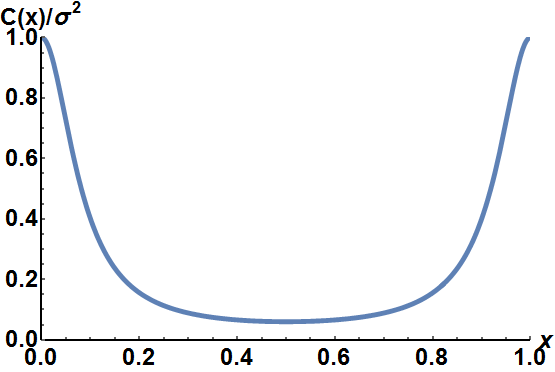
\includegraphics[width=.45\textwidth]{figs/cx.png}\hfill
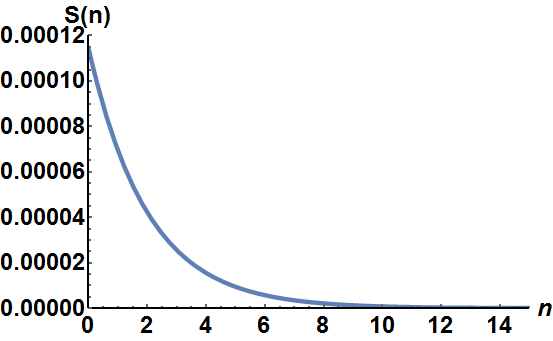
\includegraphics[width=.45\textwidth]{figs/sn.png}
\end{figure}
Recall from~(\ref{cor}) when $x=0$, the covariance function reduces to the definition
of variance. We find
\begin{align}
\begin{split}\label{a}
\sigma^2&= \alpha \frac{e^{2L}-1}{e^{2L}-2\cos(0)e^L+1}\\
\alpha &=\sigma^2 \frac{e^{2L}-2e^{L} +1}{e^{2L}-1}\\
\alpha &=\sigma^2
\frac{(e^{L}-1)^2}{(e^{L}-1)(e^{L}+1)}\\
\alpha &= \sigma^2 \tanh(L/2).
\end{split}
\end{align}
The parameter $\alpha$ is now defined in terms of the variance
$\sigma^2$ of $\xi(x)$. Such a function $C(x)$ is demonstrated in Figure~\ref{fig:correlation}
for various values of $L$.
\begin{figure}[htp]
\caption[The correlation function $C(x)$]{The correlation function
  $C(x)$ for $L \in \{0.1,0.5,1\}$. For small $L$
  (leftmost graph), the correlation is stronger between iterates than for large $L$
  (rightmost graph).}\label{fig:correlation}
\centering
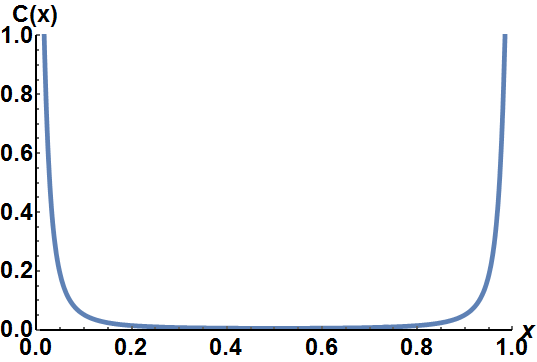
\includegraphics[width=.3\textwidth]{figs/correlation_L01.png}\hfill
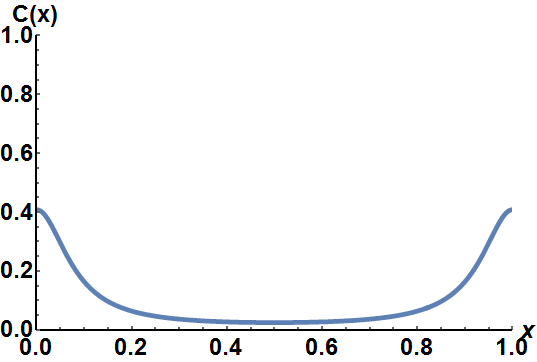
\includegraphics[width=.3\textwidth]{figs/correlation_L05.png}\hfill
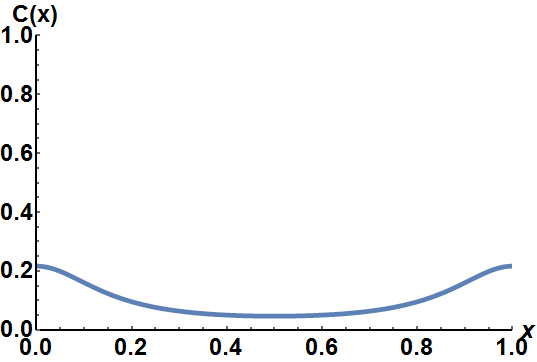
\includegraphics[width=.3\textwidth]{figs/correlation_L1.png}
\end{figure}

Recall Theorem~\ref{thm:fp} stipulates if $x \in D$, then $f(D) \subset
D$ in order for a fixed point to exist. Furthermore, for $[0,1]$ to be an invariant set of $f$, $R(x)$
must be bounded within $[0,4]$, as specified in~(\ref{logmap}). Without enforcing this condition
on~(\ref{Sn}), iterates on~(\ref{randlogmap}) would leave $[0,1]$. One way to accomplish this is to bound
the distribution of $\hat{\xi}_n$ from~(\ref{fs1}). Suppose the probability density
function for $\hat{\xi}_n$ is nonzero only in the complex square centered at the
origin with side length $2M_n$. Thus, $|a_n|,|b_n| \leq M_n$, and for a fixed $r$, we
can bound $\ln(R(x))$ using~(\ref{R}) and~(\ref{fs1})
\begin{align}
\begin{split}\label{bdnr}
|\ln(R)-\ln(r)|&\leq |\max_{R\in [0,4]}\ln(R) - \ln(r)|=\ln(4/r)\\
|\ln(R)-\ln(r)|&\leq \sum_{n\in \mathbb{Z}}|\hat{\xi}_n| \\
&\leq M_0+2\sum_{n=1}^\infty M_n\\
&\leq \ln(4/r).
\end{split}
\end{align}
The sequence of side lengths $M_n$ must be summable. 
\begin{figure}[!h]
\caption[Uniform Distribution over a Square Region]{The probability
  density function of $\hat{\xi_n}$ is uniformly distributed across
  this square region, centered at the origin. The square region has
  side length $2M_n$ and area $4M_n^2$.}\label{fig:square}
	\begin{center}
		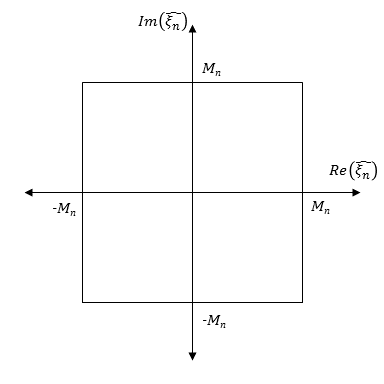
\includegraphics[scale=0.7]{figs/square.png}
	\end{center}
\end{figure}
Suppose $\hat{\xi}_n$ is uniformly distributed, so 
\begin{equation}\label{eq:square}
   h(\hat{\xi}_n) =h(a,b)= \left\{
     \begin{array}{lr}
       \frac{1}{4 M_n^2} & |a_n|,|b_n| \leq M_n\\
       0 & |a_n|,|b_n| > M_n\\
     \end{array}
   \right.
\end{equation} 
where $h:\mathbb{C}\to [0,1]\in \mathbb{R}$ is the probability density
function of $\hat{\xi}_n$. Figure~\ref{fig:square} shows the complex
region where $h(a,b)$ is nonzero. Notice that by this restriction on
$\hat{\xi}_n$, the random variable $R(x)$ is no longer ensured to be log-normal. The
sum of independent uniform random variables does not necessarily tend to a normal
distribution (by the Central Limit Theorem), since the variables are
not identical. The Central Limit Theorem states~\cite{ross}

\begin{singlespacing}
\begin{theorem}
Let $X_1, X_2, ...$ be a sequence of independent and identically
distributed random variables, each having mean $\mu$ and variance
$\sigma^2$. Then the distribution of
\begin{equation*}
\frac{X_1+...X_n-n\mu}{\sigma \sqrt{n}}
\end{equation*}
tends to the standard normal as $n \to \infty$.
\end{theorem}
\end{singlespacing}
To find the relationship between $S(n)$ and
$M_n$, recall that $S(n)$ is defined as the variance of the
log-fluctuations~(\ref{Sn}). Then, 
\begin{align}
\begin{split}\label{Mn}
S(n)&=E[|\hat{\xi}_n|^2] = E[a^2+b^2]\\
 &= \frac{1}{4M_n^2}\int_{-M_n}^{M_n}\int_{-M_n}^{M_n}a^2+b^2\,da\,db\\
&=\frac{2}{3}M_n^2\\
M_n&=\sqrt{\frac{3}{2}S(n)}.
\end{split}
\end{align}
Finally, using the expression for $\alpha$~(\ref{a}), the
expression for $M_n$~(\ref{Mn}), and the sum from~(\ref{bdnr}), let
\begin{align*}
A = M_0+2\sum_{n=1}^\infty M_n \leq \ln(4/r).
\end{align*}
Then, we find
\begin{align*}
\begin{split}
A &=\left(\sqrt{\frac{3}{2}\alpha} +
2\sqrt{\frac{3}{2}\alpha}\sum_{n=1}^{\infty}e^{-Ln/2}\right) \\
&= \sqrt{\frac{3}{2}}\alpha\left(1+ \frac{2e^{-L/2}}{1-e^{-L/2}} \right)\\
&= \sigma\sqrt{\frac{3}{2}}
\sqrt{\tanh(L/2)}\left(\frac{e^{L/2}+1}{e^{L/2}-1} \right)\\
&= \sigma \sqrt{\frac{3}{2}}\frac{\sqrt{\tanh(L/2)}}{\tanh(L/4)} \leq \ln(4/r).\\
\end{split}
\end{align*}
Thus, the standard deviation $\sigma$ must be bounded from below by
zero and from above by
\begin{align}\label{sigma}
0<\sigma \leq \ln(4/r)\sqrt{\frac{2}{3}}\frac{\tanh(L/4)}{\sqrt{\tanh(L/2)}}.
\end{align}
Figure~\ref{fig:R} is a sample realization of a function $R(x)$ that
behaves according to~(\ref{sigma}).
\begin{figure}[!h]
\caption[The function $R(x)$]{The function $R:[0,1]\to [0,4]$ where
  $\sigma=0.0386, L=0.1, r=3.5, N=100$}\label{fig:R}
	\begin{center}
		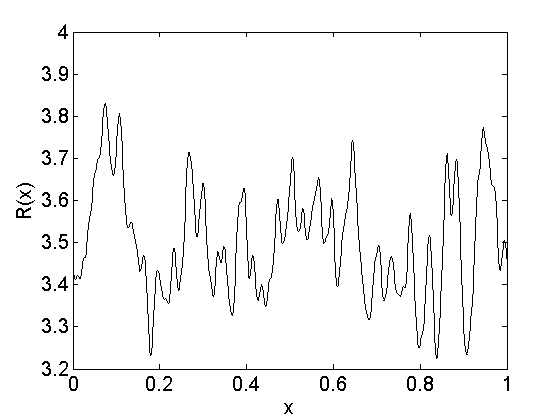
\includegraphics[scale=0.6]{figs/xi.png}
	\end{center}
\end{figure}

In summary, for each realization of the random logistic map,
we have uniform random variables $a_n,b_n \sim Unif(-M_n,M_n)$ that correspond to the
Fourier modes $n$ of $\xi(x)$ from~(\ref{fs2}) whose bounds are set by
$M_n= \sqrt{\frac{3}{2}S(n)}$, where $S(n)=\alpha e^{-L|n|}$, the
spectral density, was chosen to decay exponentially fast. $\alpha = \sigma^2 \tanh(L/2)$ is a normalization constant for the corresponding
correlation function $C(x)$, where the standard deviation $\sigma$
must be bound according to~(\ref{sigma}) in order to restrict $R(x)$
to $[0,4]$ to ensure $[0,1]$ is an invariant set of
$f$. Figure~\ref{fig:envelope} depicts rough estimates\footnote{The
  maxima and minima over 500 samples were recorded and plotted in
  these figures.} of upper and lower bounds for the random logistic
map for various sets of parameters. 
\begin{figure}[htp]
\caption[Upper and lower bounds on the random logistic map]{A coarse
  demonstration (500 samples) of the upper and lower bounds of the random logistic
  map. Sample realizations are shown in red. From left to right:
  $\{\sigma=0.1093,r=2.7,L=0.9,N=112\}, \{\sigma=0.0086,r=3.5,L=0.05,N=200\},\{\sigma=0.0071,r=3.7,L=0.1,N=100\}$
  }\label{fig:envelope}
\centering
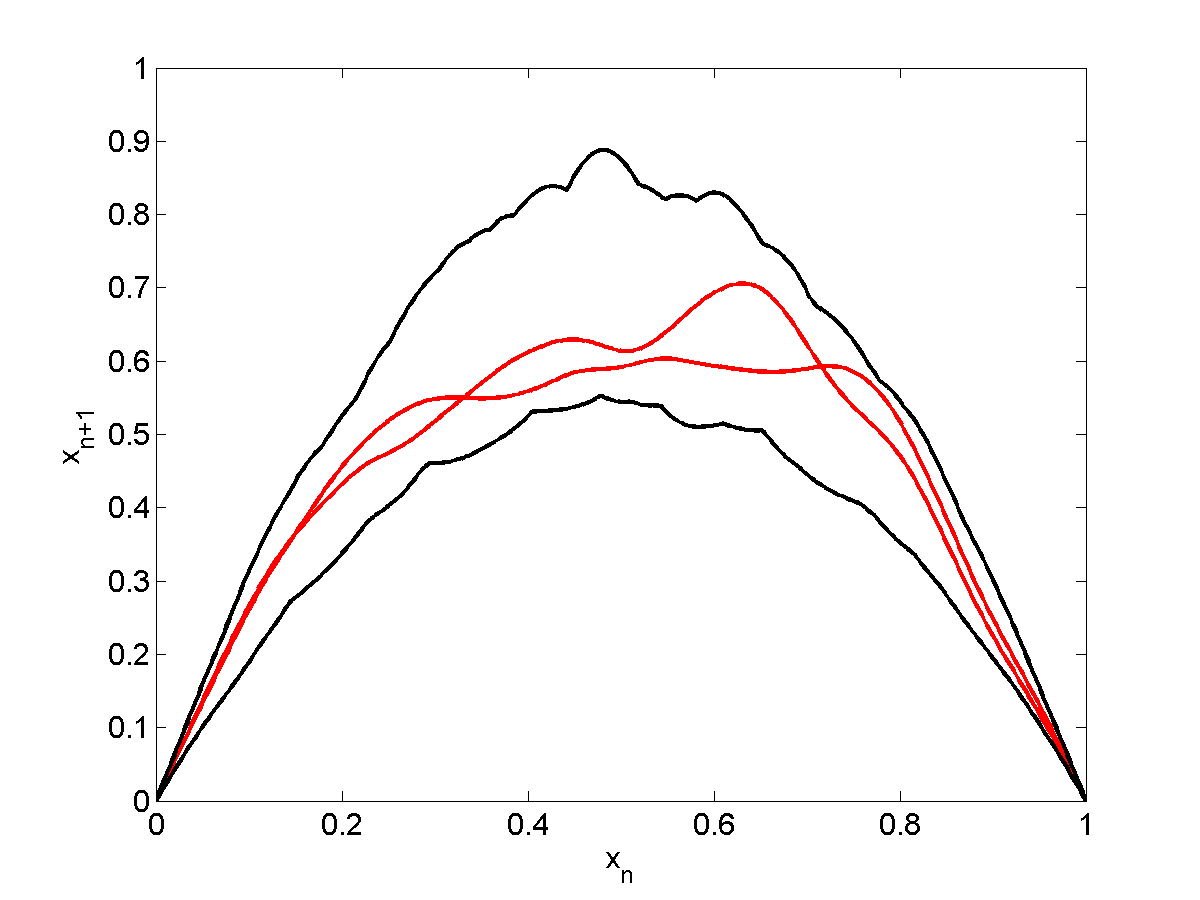
\includegraphics[width=.3\textwidth]{figs/envelope_500_r27_L09.png}\hfill
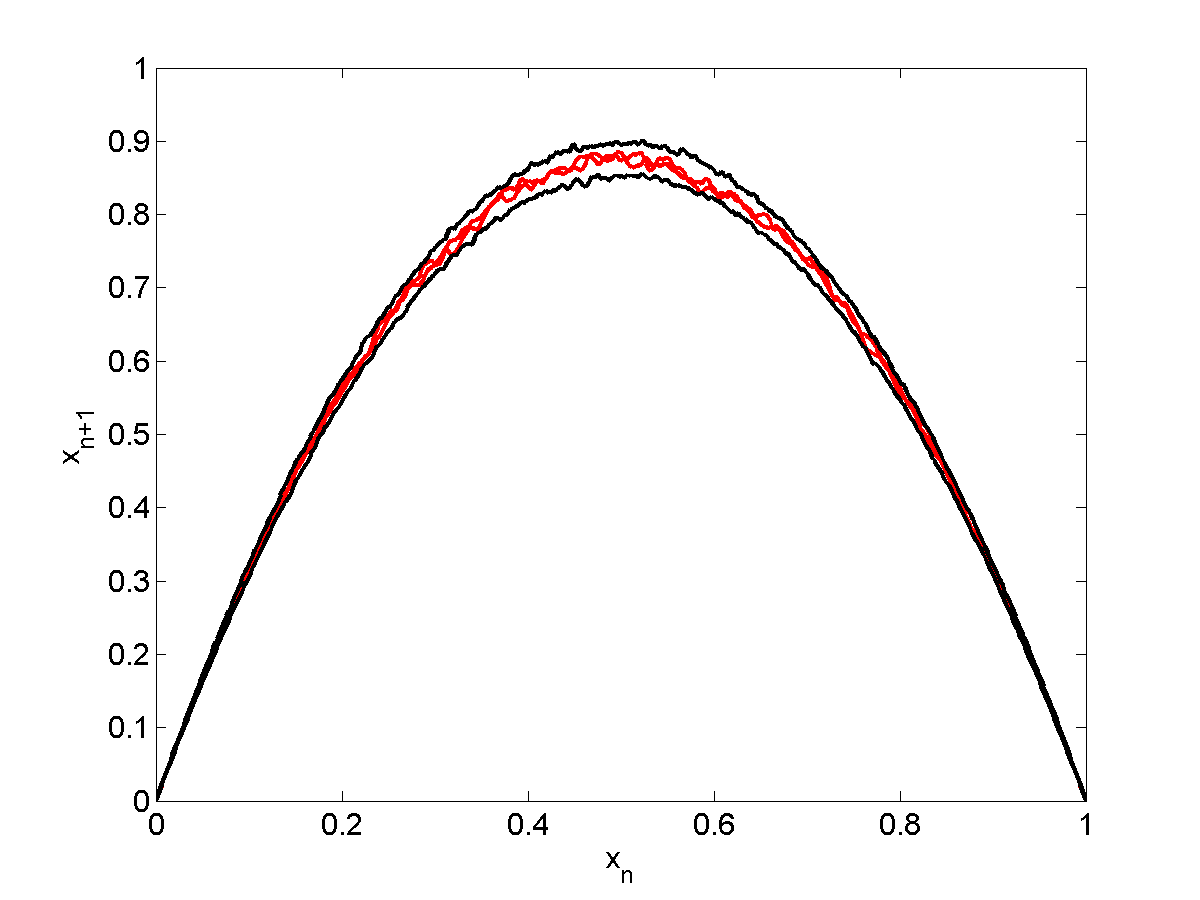
\includegraphics[width=.3\textwidth]{figs/envelope_500_r35_L005.png}\hfill
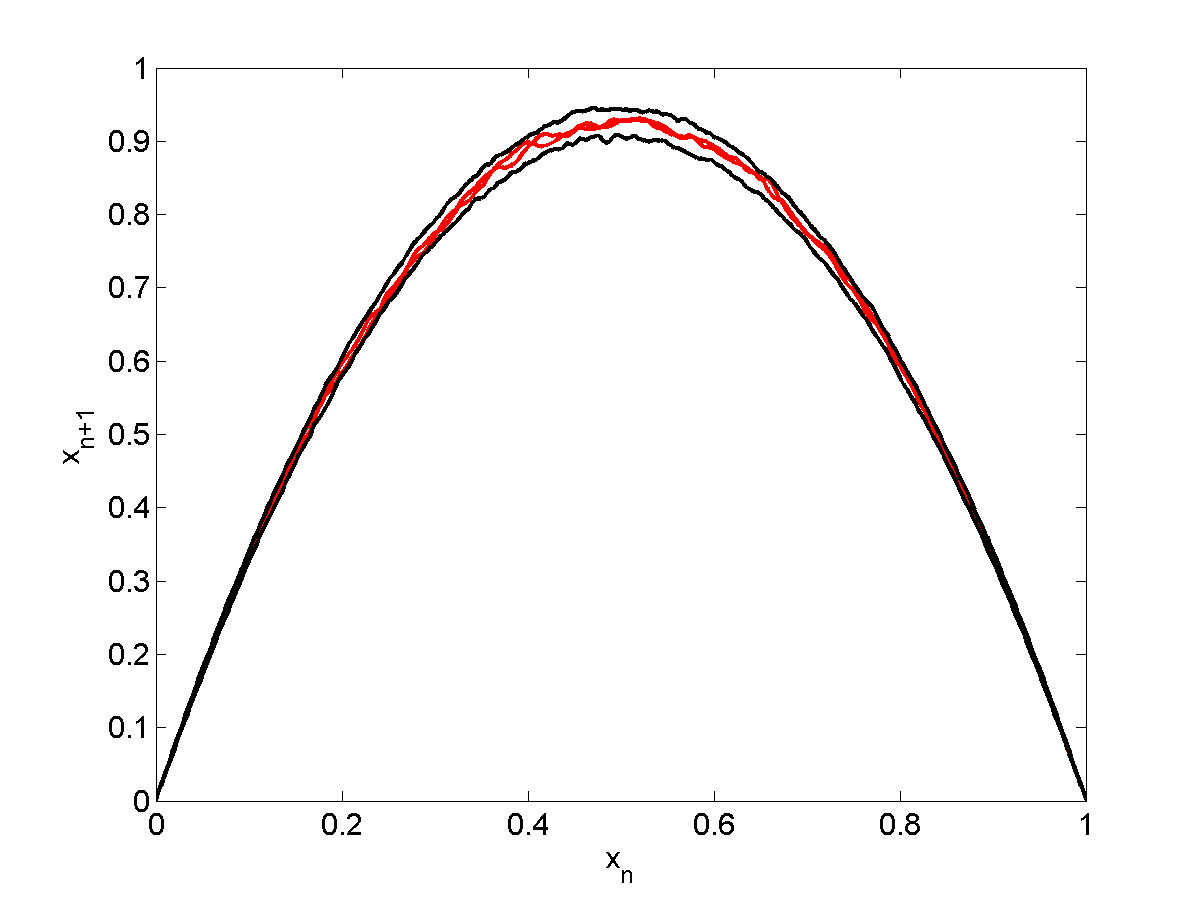
\includegraphics[width=.3\textwidth]{figs/envelope_500_r37_L01.png}
\end{figure}

\section{Circle Map}
The circle map is another
recursive expression whose deceivingly simple form gives way to complicated behavior. It was used to
understand the dynamics of a kicked rotor by Vladimir
Arnold, who is credited for discovery of what are now called the Arnold Tongues, which are
regions of stable periodic motion in the bifurcation diagram of the
map. Generally, a degree-one circle map takes the form
\begin{align*}
x_{n+1}&=f(x)=x_n + \omega + g(x_n) \mod 1\\
g(x_n)&=g(x_n + 1),
\end{align*}
where the angle $x$ has been normalized so that its range is $[0,1)$
instead of $[0,2\pi )$, $\omega$ is the driving frequency of the map, and
$g(x)$ is the nonlinear component of the recursion~\cite{rasband}. The
parameter $\omega$ represents the frequency of the driving
force, which is the external force applied to the
rotor. We define the circle $S^1$ as $\mathbb{R} \setminus
\mathbb{Z}$. The \textbf{degree} of a map $f:S^1 \to S^1$ is the integer
deg($f$) given by 
\begin{align*}
\deg(f) = F(1) - F(0),
\end{align*}
where $F:\mathbb{R} \to \mathbb{R}$ is the lift of the
map. $F$ is called the \textbf{lift} of $f$ if
\begin{align*}
w \circ F = f \circ w,
\end{align*}
where $w:\mathbb{R} \to S^1$ is defined as
\begin{equation*}
w(x) = e^{2\pi i x} = \cos(2\pi x) + i\sin(2\pi x).
\end{equation*}
$w$ wraps $\mathbb{R}$ around the circle $S^1$ without critical
points~\cite{devaney}. $w$ is many-to-one, therefore it is not a topological conjugacy
between $F$ and $f$. Since $f$ is an orientation
preserving diffeomorphism of the circle, it follows that the lift of a $f$ must be
monotonic increasing, i.e. $F'(x)>0$.

\begin{singlespacing}
\begin{definition}
Let $f:I \to J$. The function $f(x)$ is a homeomorphism if $f(x)$ is
one-to-one, onto, and continuous, and $f^{-1}(x)$ is also continuous~\cite{devaney}.
\end{definition}
\begin{definition}
Let $f:I\to J$. The function $f(x)$ is a $C^r$-diffeomorphism if
$f(x)$ is a $C^r$-homeomophism such that $f^{-1}(x)$ is also $C^r$~\cite{devaney}. 
\end{definition}
\end{singlespacing}

A phenomenon of \textbf{mode-locking} may occur in the map,
where after $q$ iterations, the new angle differs from the initial
value of $x$ by exactly $p \in \mathbb{Z}$
\begin{align*}
x_{n+q}=x_n+p.
\end{align*}
The \textbf{rotation number} of the orbit is an important invariant of
the circle map because it measures the average amount of points
rotated by an iteration of the map. Essentially, it gives an idea of
whether $f$ has periodic orbits.

\begin{singlespacing}
\begin{definition}\label{rho}
The rotation number of $f$, $\rho(f)$, is the fractional part of
$\rho_0(F) = \lim_{n \to \infty} \frac{|F^n(x)|}{n}$ for any lift $F$ of $f$. That is, $\rho(f)$ is the unique
number in [0,1) such that $\rho_0(F)-\rho$ is an integer~\cite{devaney}.
\end{definition}
\end{singlespacing}

\noindent When $\rho \in \mathbb{Q}$, the system is mode-locked. Since
$\rho$ is a rational number, it can be expressed as $p/q$, where $p,q
\in \mathbb{Z}$. The order of the periodic orbit is $q$. If $\rho$
does not exist, then the system may be in a chaotic
state. When $\rho \in \mathbb{R} \setminus \mathbb{Q}$, the orbit is
quasiperiodic. The theorem below
establishes the rotation number of the map $\rho(f)$
depends continuously on $f$, and that if $f$ is monotone, then all
orbits have the same rotation number.

\begin{singlespacing}
\begin{theorem}
Let $f:S^1 \to S^1$ be an orientation-preserving diffeomorphism with
lift $F$. Then
\begin{equation*}
\rho_0(F) = \lim_{n \to \infty} \frac{|F^n(x)|}{n}
\end{equation*}
exists and is independent of both $x$ and the lift $F$. Hence the
rotation number $\rho(f)$ is well-defined~\cite{devaney}.
\end{theorem}
\end{singlespacing}

\subsection{Deterministic case}
Arnold introduces the two-parameter example
\begin{align}\label{detcirc}
x_{n+1}= F(x_n) =  x_n + \omega - \frac{k}{2\pi}\sin(2\pi x_n),
\end{align}
which we will explore as well. (\ref{detcirc}) is the lift of the map
$f$,
\begin{align}\label{detcirc2}
f(x_n) = x_n + 2\pi \omega + k\sin(x_n).
\end{align}
In both (\ref{detcirc}) and (\ref{detcirc2}), there are two parameters: $k \in [0,\infty)$
is the coupling strength and $\omega \in [0,1]$ is the driving
frequency. When discussing $f$, we will deal exclusively with the
lift, $F$. According to Theorem~\ref{thm:fp}, existence of fixed
points depends on the condition $\forall x \in S^1, f(S^1) \subset S^1$
in~(\ref{detcirc}). Taking the modulus of~(\ref{detcirc}) will fulfill
the requirement, so we find
\begin{align*}
x_{n+1}= F(x_n) \mod 1.
\end{align*}
A stable period 2 orbit is shown in
Figure~\ref{fig:dcircstable}, and
Figure~\ref{fig:rcircunstable} shows an orbit that may have diverged.
\begin{figure}[!h]
\caption[Deterministic circle map, stable orbit]{The cobweb
  diagram (green) for a deterministic circle map (blue) with $\omega =
  0.5$ and $k=1$. The line $x_{n+1}=x_n$ is drawn in red. The orbit
  has converged to a stable period 2 after 1000 iterations. Transient iterations were removed.}\label{fig:dcircstable}
	\begin{center}
		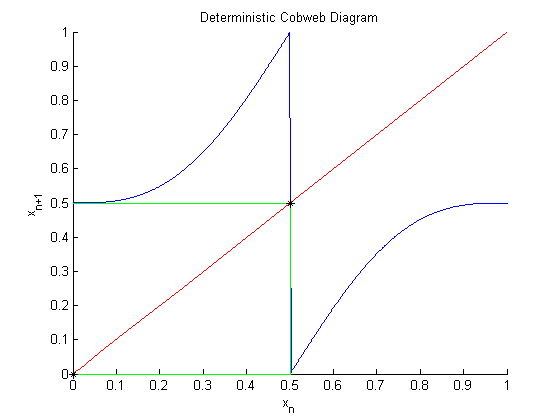
\includegraphics[scale=0.7]{figs/detcirc_cobweb_2.png}
	\end{center}
\end{figure}
\begin{figure}[!h]
\caption[Deterministic circle map, unstable orbit]{The cobweb
  diagram (green) for a deterministic circle map (blue) with $\omega =
  0.6$ and $k=1$. The line $x_{n+1}=x_n$ is drawn in red. The orbit
  appears to have diverged after 1000 iterations. Transient iterations were removed.}\label{fig:rcircunstable}
	\begin{center}
		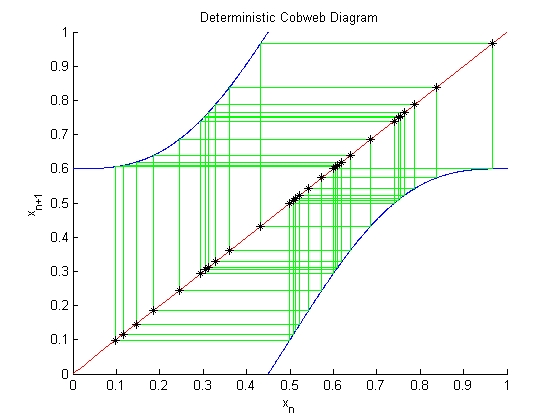
\includegraphics[scale=0.7]{figs/detcirc_cobweb_chaos.png}
	\end{center}
\end{figure}
The coupling strength $k$
controls the amplitude of the oscillations in the circle map; no
coupling is $k=0$, and the coupling increases as $k \to
\infty$. For $0 \leq k < 1$, $f$ is a diffeomorphism of $S^1$, and
when $k=1$, the map is a homeomorphism. For $k>1$, the map is no
longer one-to-one, so $\rho$ may not exist~\cite{devaney}. In contrast, $\omega$
applies a positive vertical shift to the map, which causes it to wrap around itself, due to the effects of the modulo operator. The changes in the rotation number $\rho$ as $\omega$ is
varied over [0,1] is graphically demonstrated as a Devil's Staircase
in Figure~\ref{fig:devil_det}. The graph of $\rho(\omega)$ is a Cantor
function. Cantor functions are everywhere continuous and have zero
derivative almost everywhere. The Devil's Staircase is everywhere
continuous; it is constant for
rational rotation numbers, and takes on every value in between the
rational numbers~\cite{devaney}.
\begin{figure}[!h]
\caption[The Devil's Staircase for the deterministic circle map]{The
  plot of $\omega$ vs the rotation number $\rho$ for $k=1$ results in a Devil's
  Staircase, which maps $[0,1]\to [0,1]$. Since the circle map is monotone, $\rho$ is independent of
  the initial value $x_0$. At each $\omega$, $\rho$ is either
  irrational or rational (due to the quasiperiodic cases), which results in a monotonically increasing
  "staircase." The largest steps (where $\rho$ appears constant)
  correspond with the simplest rationals.}\label{fig:devil_det}
	\begin{center}
		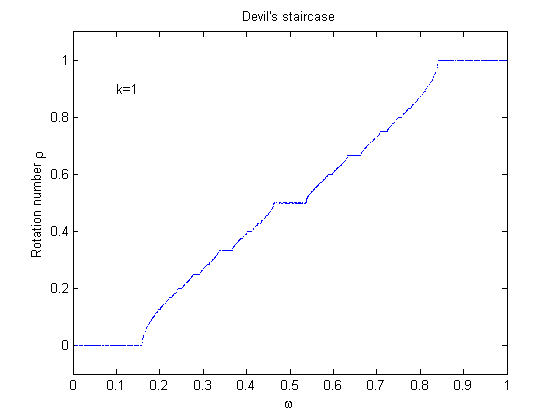
\includegraphics[scale=0.7]{figs/devil_nonrandom_k1.png}
	\end{center}
\end{figure}
The width of each "step" corresponds to the width of the Arnold
Tongues (Figure~\ref{fig:dettongues}) in the bifurcation diagram for $k$ and $\omega$ in~(\ref{detcirc}). 
\begin{figure}[!h]
\caption[The Arnold Tongues for the deterministic circle map]{A color coded
  plot of the order the of periodic orbit for values of $\omega \in [0,1]$ vs $k \in [0,1]$ creates a bifurcation diagram that looks
  like tongues. This plot samples 1000 values of $\omega$ and $k$ in [0,1].}\label{fig:dettongues}
	\begin{center}
		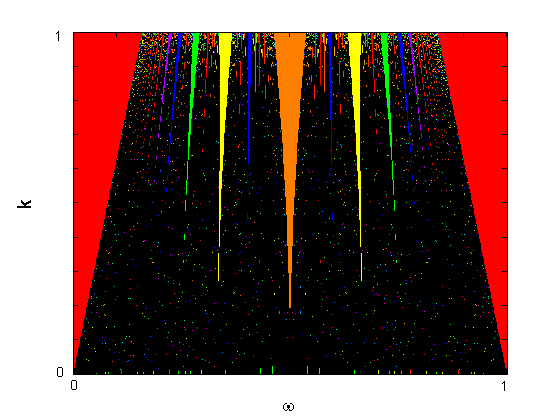
\includegraphics[scale=0.7]{figs/tongues_1000_det.png}
	\end{center}
\end{figure}
\subsection{Random case}
We will investigate a spatially random circle map of the form
\begin{align}\label{randcirc}
x_{n+1}= F(x_n) =  x_n + \Omega(x_n) - \frac{k}{2\pi}\sin(2\pi x_n),
\end{align}
where $\omega$ from~(\ref{detcirc}) has been replaced with a function
of space, $\Omega:S^1\to S^1$. In Figure~\ref{fig:rcircstable}, a realization of the
random circle map using the probability density function $h$ is shown,
where the orbit converges to a period 5 orbit. 
\begin{figure}[!h]
\caption[Random circle map, stable orbit]{The cobweb
  diagram (green) for a random realization of the circle map (blue) with $\omega =
  0.3, k=1, \alpha = 10^{-5}$. The line $x_{n+1}=x_n$ is drawn in red. The orbit
  has converged to a stable period 5 orbit. Its basin of attraction is
  $S^1$. Transient iterations were removed.}\label{fig:rcircstable}
	\begin{center}
		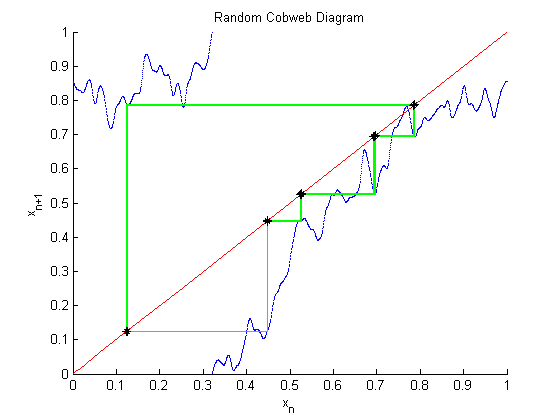
\includegraphics[scale=0.7]{figs/randcirc_cobweb.png}
	\end{center}
\end{figure}
We wish to mimic the noise in hydraulic modeling, so we
will assume that
\begin{align}\label{Omega}
\xi(x) = \ln(\Omega(x)),
\end{align}
where properties of the random variable $\xi(x)$ will be similar to those of the random logistic map. As before, a normal random variable $\xi(x)$ may be
constructed with a Fourier Series:
\begin{align}\label{fs_circ}
\begin{split}
\xi(x) &= \ln(\omega) + \sum_{n \in \mathbb{Z}}\hat{\xi_n}e^{2\pi inx}\\
&= \ln(\omega) + 2\sum^N_{n=1}a_n\cos(2\pi nx)-b_n\sin(2\pi nx).
\end{split}
\end{align}
We continue to enforce $\hat{\xi_n} = a_n + ib_n = \hat{\xi}_{-n}^*$
to keep $\xi(x) \in \mathbb{R}$. The real and imaginary parts
$(a_n,b_n)$ of $\hat{\xi}_n$ are independent with mean
$\hat{\mu}_n=E[\hat{\xi}_n]=0$ and variance $\hat{\sigma}_n^2=E[\hat{\xi}_n^2]=S_n$,
where $S_n$ is the spectral density~(\ref{spec}). The
spectral density decays exponentially, so $S_n$ in this case
takes the same form as for the random logistic map. However, since we
do not require $\Omega(x)$ of the circle map~(\ref{randcirc}) to be bounded as strictly
as $R(x)$ of the logistic map~(\ref{randlogmap}), $\alpha$ may be
chosen freely. Moreover, we use a different uniform probability density
function $\tilde{h}:\mathbb{C}\to [0,1]\in \mathbb{R}$ to ensure the
random variables $a_n,b_n$ are independent and identically distributed. 
\begin{equation}\label{eq:circh}
   \tilde{h}(\hat{\xi}_n) =h(a,b)= \left\{
     \begin{array}{lr}
       1 & |a_n|,|b_n| \leq 1\\
       0 & |a_n|,|b_n| > 1\\
     \end{array}
   \right.
\end{equation} 
Therefore, the random
variable $\xi(x)$ tends to the normal distribution, by the Central
Limit Theorem. It follows that $\Omega(x)$ is a log-normal random
variable, as desired. 

Overall, we have a much simpler set of equations for the circle map
than for the logistic map since $\Omega(x)$ is unrestricted. For each realization of the map, we choose
a set of random variables, $a_n, b_n \sim Unif(-M_n,M_n)$, that
correspond to the Fourier modes of $\xi(x)$. Their magnitudes decrease
as $M_n=\sqrt{\frac{3}{2}S_n}$ diminishes exponentially, due to the
exponential term in $S_n=\alpha e^{-L|n|}$, where $\alpha$ is a constant. 